\documentclass{article}
\usepackage{float,amsmath}
\usepackage{graphicx}
\usepackage{color}
\usepackage[letterpaper,margin=1in]{geometry}
\usepackage{hyperref}

\usepackage{etoc}

\usepackage{outlines}
\usepackage{enumitem}
\setenumerate[1]{label=\arabic*.}
\setenumerate[2]{label=\alph*.}
\setenumerate[3]{label=\arabic*.}
\setenumerate[4]{label=\roman*.}

\newcommand{\mc}{M\&C}

\hypersetup{
    colorlinks=true,
    linkcolor=blue,
    filecolor=magenta,
    urlcolor=cyan,
    pdftitle={MC Definition},
    bookmarks=true,
    pdfpagemode=FullScreen,
}

\begin{document}

\author{HERA Team}
\title{HERA Monitor and Control Subsystem Definition}
\maketitle

\section{Introduction}
HERA is an international experiment to detect and characterize the Epoch of
Reionization (EOR).  The telescope is located at the South African SKA site in
the Karoo Astronomy Reserve.  This note summarizes Monitor and Control (\mc) subsystem for HERA.

Monitor and Control has two main tasks: configuration management and real time metadata logging. Configuration management involves tracking all the physical parts of the telescope and how they are all connected. Real time metadata logging tracks the performance, settings and communications of the subsystems.

The \mc\ system is built around a database with a well documented table schema and a python software layer to provide a simple developer framework. It also includes various online daemons for monitoring things, and both a front end web-based user interface and a command-line interface to support analysis code.

Software is contained in the repository https://github.com/HERA-Team/hera\_mc.

The organization of this document is as follows: the high-level \mc\ requirements and the design specifications are in laid out in section \ref{sec:reqs}, the configuration management is described in section \ref{sec:config}, the database tables are detailed in section \ref{sec:tables} and future plans are sketched out in section \ref{sec:future}.

\section{Requirements and Specifications}
\label{sec:reqs}

\subsection{Requirements}
These were developed and established in early 2016 in discussions among the subsystem leads.

\begin{outline}[enumerate]
	\1 Ability to fully reconstruct the historical state of the system.
	\1 All interactions between subsystems must go through or be logged by \mc.
		\2 Both subsystems in an interaction are responsible for logging communications to \mc.
		\2 Subsystems in an interaction are responsible for logging communications to \mc.
	\1 Operational metadata (e.g. temperatures, correlator bit occupancies) must be logged to \mc.
	\1 High availability (\mc\ must not limit uptime of telescope).
	\1 \mc\ is a provider of information about observations to end-users and must be available to them
\end{outline}

\subsection{Design Specification}
These were developed and established in 2016 based on the requirements.

\begin{outline}[enumerate]
	\1 SQL database
		\2 DB Design principle: every logical sub group has a group of tables.  One adds tables to do more things. E.g. different versions of subsystems add new tables. Operations reference which tables they use.
		\2 This document (and appendices) will contain all table definitions.
		\2 Use careful dB design to avoid duplicated data, make table links/data relationships clear, use many-to-one and many-to-many links.
		\2 Transactions must be used to ensure DB integrity.
		\2 Must be mirrored in some fashion to observer locations.
	\1 At least one SW interface layer will be provided.
		\2 It's not required to interact with \mc.
		\2 Must support relational db (i.e. multiple column primary and foreign keys) and transactions.
	\1 Hardware
		\2 LOM capabilities
		\2 Multi-teraByte mirrored disk RAID
		\2 Backup machine available on site
\end{outline}



% --------------------------- Configuration Management ------------------------------------------------------

\section{Configuration Management}
\label{sec:config}

The HERA array/part configuration management database is a set of five tables within the larger hera\_mc database, which is maintained on-site in the Karoo.  The tables are detailed in the Appendix,
but they are:

\begin{center}
\begin{tabular}{l l l}
         {\bf psql table} & {\bf in python file}  &  {\bf with class name} \\
	geo\_location 	& hera\_mc/geo\_location.py & GeoLocation \\
	station\_type 	& hera\_mc/geo\_location.py & StationType \\
	parts 	& hera\_mc/cm\_part\_connect.py & Parts \\
	part\_info 	         & hera\_mc/cm\_part\_connect.py & PartInfo \\
	connections 	& hera\_mc/cm\_part\_connect.py & Connections \\
	cm\_version      & hera\_mc/cm\_transfer.py & CMVersion\\
	apriori\_antenna & hera\_mc/cm\_part\_connect.py & AprioriAntenna\
\end{tabular}
\end{center}

The databases are structured primarily around {\em parts} and {\em connections}.  {\em Parts} are meant to be single items that, in theory at least, are a thing that can be replaced as a unit.
{\em Connections} define {\em ports} on a given part and connect two ports together.  By convention, HERA part numbers ({\tt hpn}) are all upper case and ports are all lower case.

All parts and connections are timed in that they have a start and stop time of operation.  If stop is {\tt None}, then it is active (it is given a date in the relatively far future).  There are currently two special parts (one at each end of the signal chain) that are ``geo\_located'' parts and have entries in the geo\_location table: {\bf station} and {\bf node}.

Parts are hooked together via connections of their ports, as defined in the connection table.   There are two types of connections:  (1) "hookup" connections and (2) "physical" connections, discussed below.

To capture antenna status, an {\em a priori} antenna status table has been defined to facilitate a work flow to incorporate new antennas into the array and capture and known recalcitrant antennas.  The table provides an enumerated status for each antenna station.  The status is one of:
\begin{itemize}\setlength\itemsep{-.3em}
	\item not\_connected
	\item needs\_checking
	\item known\_bad
	\item passed\_checks
\end{itemize}


\subsection{Operation Workflow}
The work flow in this context relates to antenna migration between one of the {\em a priori} status states above.  It is handled by the operations team, which will review the situation on a roughly monthly cadence.   Initially, all antennas are given a ``not\_connected" status.  When they are connected, they will be moved to the ``needs\_checking" state.  In operation, at each review an antenna may then be moved into one of the states of:  ``needs\_checking", ``known\_bad", or ``passed\_checks".  Ideally, an antenna will not remain in the ``needs\_checking" state for more than one iteration of the review cycle.
In pipeline operations, the {\em a priori} status state is read by the real-time processing (RTP) system.  Antennas in the ``passed\_checks" (and generally the ``needs\_checking") states are processed and passed on.

\subsection{Signal Chain Hookup Connections}
Hookup connections are those that uniquely map the signal chain from the antenna to the node, including the specific correlator input.  These connections are defined in the file {\tt cm\_part\_connect} as the {\tt full\_connection\_path}.  These are the connections used to generate the correlator hookup.
The signal chain hook-up is given below and shown in Fig. \ref{fig:hookup}, shown in black.  The list below describes the hookup connections.
\begin{itemize}\setlength\itemsep{-.3em}
	\item {\bf Station}: geo\_located position.  See prefixes in table station\_type ({\em e.g.} {\tt HH} for herahex)
	\item {\bf Antenna}:  This is also the correlator number which now matches station number.  {\tt{\bf A}\{\#\}}
	\item {\bf Feed}:  element feed (Vivaldi).  {\tt {\bf FDV}\{\#\}}
	\item {\bf FEM}:  front-end module. {\tt {\bf FEM}\{\#\}}
	\item {\bf Node bulkhead plate}:  bulkhead plate on node.  {\tt {\bf NBP}\{\#\}}
	\item {\bf PAM}:  post-amp module in node. {\tt {\bf PAM}\{\#\}}
	\item {\bf SNAP}:  digitizer/channelizer in node. {\tt {\bf SNP}\{\#\}}
	\item {\bf Node}: field-deployed node as a part {\tt {\bf N}\{\#\}}
	\item {\bf Node}:  geo\_located position for node as a station {\tt {\bf ND}\{\#\}}
\end{itemize}

\begin{figure}[H]
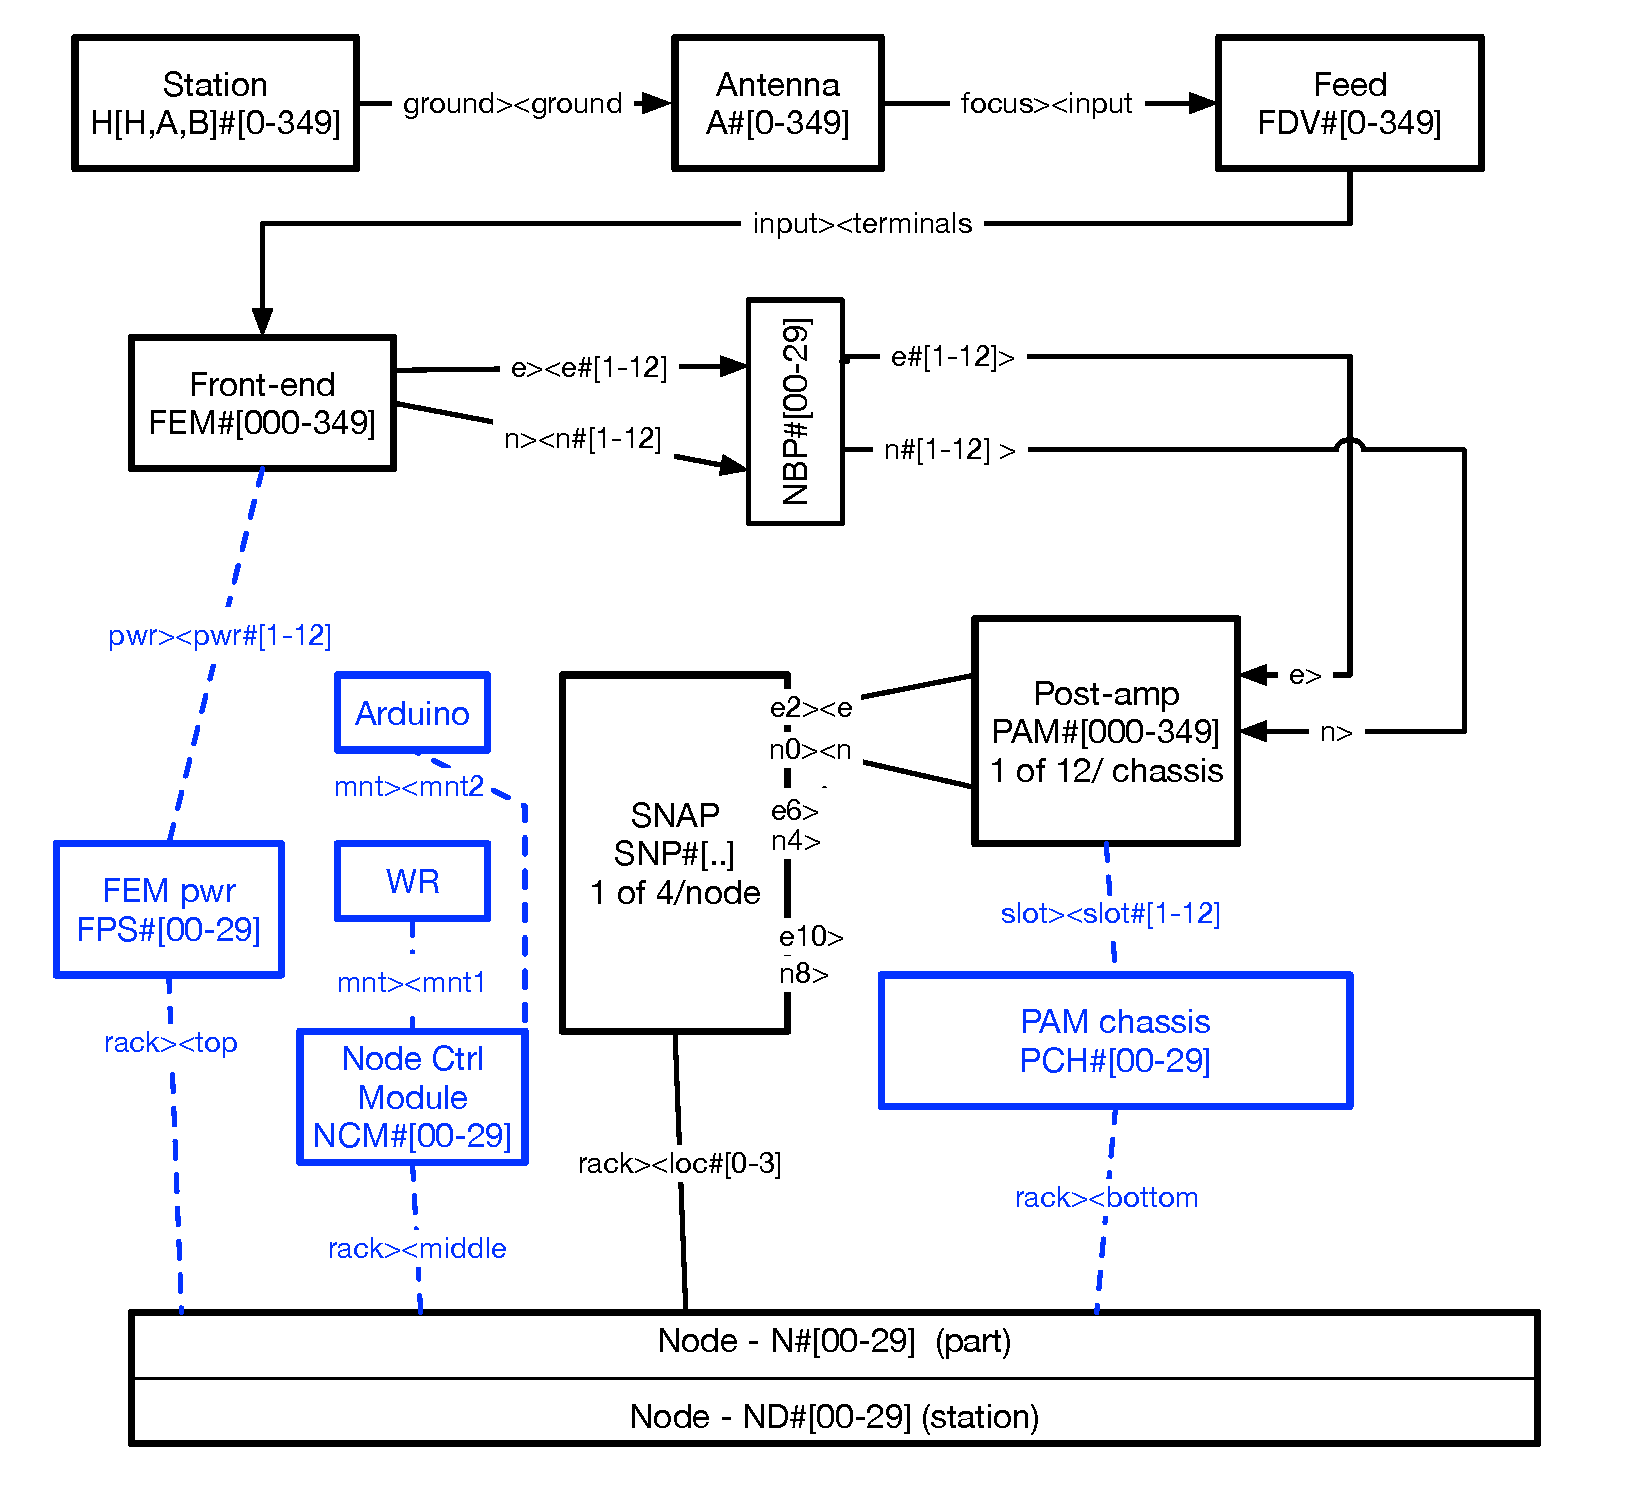
\includegraphics[width=0.8\textwidth]{hookup.pdf}
\centering
\caption{Block diagram of hookup.  The line labels indicate the port names/connections.}
\label{fig:hookup}
\end{figure}

\subsection{Physical Connections}
Possibly not the most aptly named "physical" connections are other connections that we wish to track for various operational reasons (e.g. tracing a problem to a single PAM chassis etc).  Unlike for hookup connections, these are not defined anywhere and new ones may be included as needs arise.  They are shown in Fig. \ref{fig:hookup} in blue.

\subsection{Package Modules}
This section provides a high-level overview of the python configuration management package modules within hera\_mc that are called from scripts or used in interactive sessions.
\vspace{0.5cm}

\begin{tabular}{l p{12cm}}
{\bf geo\_location.py} & Defines {\tt station\_type} and {\tt geo\_location}.  Provides update utility for {\tt geo\_location}.  Contains {\tt is\_in\_geo\_location} and {\tt is\_in\_connections}. \\ \hline
{\bf geo\_handling.py} & Contains myriad defs that handle various geo functionalities.\\ \hline
{\bf cm\_part\_connect.py} & Defines {\tt parts\_paper}, {\tt part\_info}, and {\tt connections}.  Provides update utilities for {\tt parts\_paper} and {\tt connections}. Contains {\tt \_\_get\_part\_revisions}. \\ \hline
{\bf cm\_table\_info.py} & Has mapping and order of tables and classes for initialization. \\ \hline
{\bf cm\_handling.py} & Defines the {\tt Handling} class to handle various configuration management functionalities.\\ \hline
{\bf cm\_health.py} & Contains modules that check for various cm errors or warnings \\ \hline
{\bf cm\_transfer.py} & Contains myriad defs that help package and initialize the cm tables.\\ \hline
{\bf cm\_part\_revisions.py} & Contains myriad defs that deal with finding revision numbers etc.\\ \hline
{\bf cm\_hookup.py} & Defines the {\tt Hookup} class to help determine and show the full part hookup.\\ \hline
{\bf cm\_dataview.py} & Contains various methods to display cm information.\\ \hline
{\bf cm\_utils.py} & Contains various defs called by other modules.\\ \hline
{\bf cm\_sysutils.py} & Various system-wide modules.
\end{tabular}

\subsection{Scripts}
\label{sec:scripts}
This section provides a high-level overview of the high-level scripts:  {\tt geo.py},  {\tt parts.py} and {\tt hookup.py}.

\subsubsection{Geographical Information:  {\tt geo.py fg\_action --arguments}}

Has various plotting/printing options for station information.  {{\tt fg\_action} is the "foreground action", that is the locations that will get printed and shown on top if plotting.
Available foregrounds are (note you need the first letter only):
\begin{itemize}\setlength\itemsep{-.3em}
\item {\tt a[ctive]}:  those antennas that are shown as fully hooked up through the correlator
\item {\tt i[nstalled]}:  those antennas whose structure is installed
\item {\tt p[osition] <csv-list>}:  specified antennas in csv-list (e.g. HH1,HH4)
\item {\tt c[ofa]}:  the center-of-the-array
\item {\tt s[ince]}:  antennas installed since date/time supplied in arguments
\item {\tt n[one]}:  no foreground, will just show the background (or nothing if not plotting)
\end{itemize}

Arguments are:
\begin{itemize}\setlength\itemsep{-.3em}
\item {\tt -b, --background}:  antenna types as background - none, installed, layers, all (note:  layers=all+station-types+foreground)
\item {\tt -g, --graph}:  show the graph
\item {\tt -f, --file}: if included, will write out foreground to that filename
\item {\tt --date, --time}:  date/time to use for foreground
\item {\tt -x, -y}:  specifiy x and y axes to use (n, e, z)
\item {\tt -t, --station-types}:  station-types to use in foreground retrieval
\item {\tt --label}:  what to use as label for plot.
\end{itemize}

\subsubsection{Part/Connection Information: {\tt parts.py action --arguments}}
Has various printing options for part information (part info, connections, hookup, types, etc). {\tt parts.py info} will print out some helpful script info. Available actions are (note you only need the first 2 letters only):
\begin{itemize}\setlength\itemsep{-.3em}
\item {\tt info}:   provides information on the script
\item {\tt part\_info}:   provides a summary of given part(s)
\item {\tt conn\_info}:   provides a summary table of parts connected to given part(s)
\item {\tt rev\_info}:  provides a summary of revisions to given part(s)
\item {\tt types}:  prints a summary table of part types
\item {\tt check\_rev}:  checks whether a given revision of a part exists
\item {\tt overlap\_check}:  checks that the given part doesn't have overlapping revisions.
\end{itemize}

Arguments are:
\begin{itemize}\setlength\itemsep{-.3em}
\item {\tt -p, --hpn}:  hera part number (hpn), a csv-list of them, or partial hpn
\item {\tt -r, --revision}: part revision - can be active, last, all or specific (defaults to active)
\item {\tt --port}: a specific port to find, or all
\item {\tt -e, --exact-match}: forces an exact match to the hpn (so 'HH1' doesn't return all teens and hundreds
\item {\tt --notes}: will display part notes as opposed to the part table (only for action=part\_info)
\item {\tt --sort\_notes\_by}:  if {\tt --notes}, specifies how they are sorted on display, either by part or posting time (post)
\item {\tt -v, --verbosity}:  how much to show, -v, -vv, -vvv
\item {\tt --date, --time}:  date/time to use for active parts/connections etc
\item {\tt --notes\_start\_date, --notes\_start\_time}:  date/time to use for filtering {\tt --notes}
\end{itemize}

\subsubsection{Cascaded Connection Information:  {\tt hookup.py --arguments}}
Displays the signal chain hookup information.

Arguments are:
\begin{itemize}\setlength\itemsep{-.3em}
\item {\tt -p, --hpn}:  hera part number (hpn), a csv-list of them, or partial hpn
\item {\tt -r, --revision}: part revision - can be active, last, all or specific (defaults to active)
\item {\tt --port}: a specific port to find, or all
\item {\tt -e, --exact-match}: forces an exact match to the hpn (so 'HH1' doesn't return all teens and hundreds
\item {\tt --date, --time}:  date/time to use for active connections
\item {\tt -f, --force-new}:  forces a new hookup cache file to be written for search
\item {\tt -c, --cache-info}:  display information about the cache file
\item {\tt --force-specific}:  subtly different than force new, based on the searched for keys
\item {\tt --state}:  hookup state to show:  full or all
\item {\tt --hookup-cols}:  specify which columns to print out
\item {\tt --levels}:  show correlator levels (currently not functional)
\item {\tt --hide-ports}:  don't show the ports in hookup table
\item {\tt --revs}:  show the revs in the hookup table
\item {\tt delete-cache-file}:  deletes the local cache file
\end{itemize}

% --------------------------- Table Definitions ------------------------------------------------------
\newpage

\section{Table Definitions}
\label{sec:tables}

\vspace{5mm}
\etocsettocstyle{}{}
\localtableofcontents
\newpage

The formatting of the tables is as follows:
\begin{itemize}\setlength\itemsep{-.3em}
	\item {\bf Bold font} = primary key
	\item {\em Italics} = foreign\_key.
	\item * = NotNull entries
\end{itemize}


\subsection{Observations}
\subsubsection{hera\_obs}
This is the primary observation definition table. It is written to by the correlator.

\begin{center}
 \begin{tabular}{| p{4cm} | p{2cm} | p{10cm} |}
 \hline
 {\bf Column} & {\bf Type}  & {\bf Description} \\ [0.5ex]  \hline\hline
 \textbf{obsid} & long integer & start time in floor(GPS) seconds. GPS start adjusted to be within 1 second of LST to lock observations to LST for the night \\ \hline
 starttime & double & start time in gps seconds. The start time to full accuracy of the beginning of integration of first visibility \\\hline
 stoptime & double & stop time in gps seconds. The stop time to full accuracy of the end of integration of last visibility \\\hline
 jd\_start & double & start time in JD. Calculated from starttime, provides a quick way to filter on JD times. \\\hline
 lst\_start\_hr & double & decimal hours from start of sidereal day. Calculated from starttime, provides a quick search for matching LSTs \\\hline
 \end{tabular}
\end{center}

\subsection{Common tables}
\subsubsection{server\_status (template)}
\label{sec:server_status}
Common table structure for server status info. \textbf{Note: There is no table named server\_status. This is the structure used for several subsystem tables named \textless subsystem\textgreater\_server\_status}.
\begin{center}
 \begin{tabular}{| p{4cm} | p{2cm} | p{10cm} |}
\hline
 {\bf Column} & {\bf Type}  & {\bf Description} \\ [0.5ex]  \hline\hline
 \textbf{hostname} & string &  name of server \\ \hline
 \textbf{mc\_time} & long & time report received by \mc\ in floor(gps seconds) \\ \hline
 ip\_address & string & IP address of server (how should we handle multiples?) \\\hline
mc\_system\_timediff & float & difference between \mc\ time and time report sent by server in seconds \\\hline
num\_cores & integer & number of cores on server \\\hline
cpu\_load\_pct & float & CPU load percent = total load / num\_cores, 5 min average  \\\hline
uptime\_days & float & server uptime in days  \\\hline
memory\_used\_pct & float & percent of memory used, 5 min average  \\\hline
memory\_size\_gb & float & amount of memory on server in GB \\\hline
disk\_space\_pct & float & percent of disk used  \\\hline
disk\_size\_gb & float & amount of disk space on server in GB \\\hline
network\_bandwidth\_mps & float & Network bandwidth in MB/s, 5 min average. Can be null \\\hline
\end{tabular}
\end{center}

\subsubsection{subsystem\_errors}
Subsystem errors/issues
\begin{center}
 \begin{tabular}{| p{4cm} | p{2cm} | p{10cm} |}
\hline
 {\bf Column} & {\bf Type}  & {\bf Description} \\ [0.5ex]  \hline\hline
\textbf{id} & long & auto-incrementing error id\\ \hline
time & long & error report time in floor(gps seconds)\\ \hline
subsystem & string & name subsystem with error (e.g. `librarian', `rtp')\\ \hline
mc\_time & long & time report received by \mc\ in floor(gps seconds) \\ \hline
severity & int & integer indicating severity level, 1 is most severe \\ \hline
log & text & TBD on format, either a message or a file with the log \\ \hline
\end{tabular}
\end{center}


\subsubsection{daemon\_status}
Status of \mc\ daemons that monitor various subsystems.
\begin{center}
 \begin{tabular}{| p{4cm} | p{2cm} | p{10cm} |}
\hline
 {\bf Column} & {\bf Type}  & {\bf Description} \\ [0.5ex]  \hline\hline
\textbf{name} & string & daemon name\\ \hline
\textbf{hostname} & string & hostname where daemon is running (the same daemon can run on multiple hosts)\\ \hline
\textbf{jd} & integer & Julian Date. This allows for some history without keeping all history.\\ \hline
time & long & most recent status report time in floor(gps seconds)\\ \hline
status & string & most recent daemon status. One of `good' or `errored'\\ \hline
\end{tabular}
\end{center}

% --------------------------- RTP ------------------------------------------------------

\subsection{RTP Tables}
\subsubsection{rtp\_server\_status}
RTP version of the server\_status table, see \ref{sec:server_status}.

\subsubsection{rtp\_status}
High level RTP status
\begin{center}
 \begin{tabular}{| p{4cm} | p{2cm} | p{10cm} |}
\hline
 {\bf Column} & {\bf Type}  & {\bf Description} \\ [0.5ex]  \hline\hline
\textbf{time} & long & status time in floor(gps seconds)\\ \hline
status & string & status string, options TBD (might become an enum) \\\hline
event\_min\_elapsed & float & minutes elapsed since last event \\\hline
num\_processes & integer & Number of processes running  \\\hline
restart\_hours\_elapsed & float & hours elapsed since last restart \\\hline
\end{tabular}
\end{center}

\subsubsection{rtp\_process\_events}
RTP Processing events (per obsid)
\begin{center}
 \begin{tabular}{| p{4cm} | p{2cm} | p{10cm} |}
\hline
 {\bf Column} & {\bf Type}  & {\bf Description} \\ [0.5ex]  \hline\hline
\textbf{time} & long & event time in floor(gps seconds) \\ \hline
\textit{\textbf{obsid}} & long integer & observation identifier, foreign key into hera\_obs table \\ \hline
event & string & one of: queued, started, finished, error  \\\hline
\end{tabular}
\end{center}

\subsubsection{rtp\_process\_record}
RTP record of processed obsids (entry added when processing finished)
\begin{center}
 \begin{tabular}{| p{4cm} | p{2cm} | p{10cm} |}
\hline
 {\bf Column} & {\bf Type}  & {\bf Description} \\ [0.5ex]  \hline\hline
\textbf{time} & long & record time in floor(gps seconds)\\ \hline
\textit{\textbf{obsid}} & long integer & observation identifier, foreign key into hera\_obs table \\ \hline
pipeline\_list & text & concatenated list of tasks  \\\hline
git\_version & string & git version of RTP code  \\\hline
git\_hash & string & git hash of RTP code  \\\hline
\end{tabular}
\end{center}

\subsubsection{rtp\_task\_resource\_record}
RTP record of start and stop times for a task (e.g., omnical) for an obsid, as well as CPU and memory used (if available)
\begin{center}
  \begin{tabular}{| p{4cm} | p{2cm} | p{10cm} |}
\hline
 column & type & description \\ [0.5ex] \hline\hline
\textit{\textbf{obsid}} & long integer & observation identifier, foreign key into hera\_obs table \\ \hline
\textbf{task\_name} & string & name of specific task (e.g., \verb+OMNICAL+) \\ \hline
start\_time & long & start time of task in floor(gps seconds) \\ \hline
stop\_time & long & stop time of task in floor(gps seconds) \\ \hline
max\_mem & float & maximum memory, in MB, consumed by the task; nullable column \\ \hline
avg\_cpu\_load & float & average CPU load, in number of CPUs, for task (e.g., 2.00 means 2 CPUs used); nullable column \\ \hline
\end{tabular}
\end{center}



% --------------------------- Librarian ------------------------------------------------------

\subsection{Librarian Tables}
\subsubsection{lib\_server\_status}
Librarian version of the server\_status table, see \ref{sec:server_status}.

\subsubsection{lib\_status}
High level Librarian status
\begin{center}
 \begin{tabular}{| p{4cm} | p{2cm} | p{10cm} |}
\hline
 {\bf Column} & {\bf Type}  & {\bf Description} \\ [0.5ex]  \hline\hline
\textbf{time} & long & status time in floor(gps seconds) \\ \hline
num\_files & long & total number of files in librarian  \\\hline
data\_volume\_gb & float & total data volume in gigabytes  \\\hline
free\_space\_gb & float & available space in gigabytes  \\\hline
upload\_min\_elapsed & float & minutes elapsed since last file upload \\\hline
num\_processes & integer & number of running background tasks  \\\hline
git\_version & string & git version of Librarian code  \\\hline
git\_hash & string & git hash of Librarian code  \\\hline
\end{tabular}
\end{center}

\subsubsection{lib\_raid\_status}
RAID controller status
\begin{center}
 \begin{tabular}{| p{4cm} | p{2cm} | p{10cm} |}
\hline
 {\bf Column} & {\bf Type}  & {\bf Description} \\ [0.5ex]  \hline\hline
\textbf{time} & long & status time in floor(gps seconds) \\ \hline
\textbf{hostname} & string & name of RAID server \\ \hline
num\_disks & int & number of disks in RAID server  \\\hline
info & text & TBD -- various info from megaraid controller, may be several columns \\\hline
\end{tabular}
\end{center}

\subsubsection{lib\_raid\_errors}
RAID controller errors/issues
\begin{center}
 \begin{tabular}{| p{4cm} | p{2cm} | p{10cm} |}
\hline
 {\bf Column} & {\bf Type}  & {\bf Description} \\ [0.5ex]  \hline\hline
\textbf{id} & long & auto-incrementing error id\\ \hline
time & long & error report time in floor(gps seconds)\\ \hline
hostname & string & name of RAID server with error \\ \hline
disk & string & name of disk with error \\ \hline
log & text & TBD on format, either a message or a file with the log \\\hline
\end{tabular}
\end{center}

\subsubsection{lib\_remote\_status}
Network bandwidth/health to all remote librarians
\begin{center}
 \begin{tabular}{| p{4cm} | p{2cm} | p{10cm} |}
\hline
 {\bf Column} & {\bf Type}  & {\bf Description} \\ [0.5ex]  \hline\hline
\textbf{time} & long & status time in floor(gps seconds)\\ \hline
\textbf{remote\_name} & string & name of remote librarian \\ \hline
ping\_time & float & ping time in seconds \\\hline
num\_file\_uploads & int & number of files uploaded in last 15 minutes  \\\hline
bandwidth\_mps & float & bandwidth to remote in Mb/s, 15 minute average \\\hline
\end{tabular}
\end{center}

\subsubsection{lib\_files}
File creation log
\begin{center}
 \begin{tabular}{| p{4cm} | p{2cm} | p{10cm} |}
\hline
 {\bf Column} & {\bf Type}  & {\bf Description} \\ [0.5ex]  \hline\hline
\textbf{filename} & string & name of file created \\ \hline
\textit{obsid} & long integer & observation identifier, foreign key into hera\_obs table. Can be null. \\ \hline
time & long & file creation time in floor(gps seconds)\\ \hline
size\_gb & float & file size in gigabytes \\ \hline
\end{tabular}
\end{center}



% --------------------------- Correlator ------------------------------------------------------

\subsection{Correlator Tables}
The correlator tables are not all defined yet. Notes on future plans are in section \ref{sec:corr_future}.


\subsubsection{correlator\_config\_file}
List of correlator config files, which specify detailed correlator settings. All files in this table are in the Librarian.
\begin{center}
 \begin{tabular}{| p{4cm} | p{2cm} | p{10cm} |}
\hline
 {\bf Column} & {\bf Type}  & {\bf Description} \\ [0.5ex]  \hline\hline
\textbf{config\_hash} & string & unique hash for the config\\ \hline
filename & string & name of the config file in the Librarian \\\hline
\end{tabular}
\end{center}

\subsubsection{correlator\_config\_status}
Config status of the correlator, i.e. which config file is being used by the correlator.
\begin{center}
 \begin{tabular}{| p{4cm} | p{2cm} | p{10cm} |}
\hline
 {\bf Column} & {\bf Type}  & {\bf Description} \\ [0.5ex]  \hline\hline
\textbf{time} & long & time of the config status in floor(gps seconds)\\ \hline
\textit{config\_hash} & string & hash for the config in use, foreign key into correlator\_config\_file table.\\ \hline
\end{tabular}
\end{center}


\subsubsection{correlator\_control\_state}
State of control knobs in correlator.
\begin{center}
 \begin{tabular}{| p{4cm} | p{2cm} | p{10cm} |}
\hline
 {\bf Column} & {\bf Type}  & {\bf Description} \\ [0.5ex]  \hline\hline
\textbf{time} & long & time of the control state in floor(gps seconds)\\ \hline
\textbf{state\_type} & string & type of control state, one of: `taking\_data', `phase\_switching',  `noise\_diode'.  \\ \hline
state & boolean & indicator of whether the state\_type is true or false \\\hline
\end{tabular}
\end{center}

\subsubsection{correlator\_control\_command}
Commands issued to the correlator. If the command is `take\_data' or `update\_config', there will be a matching row in the `correlator\_take\_data\_arguments' table or the `correlator\_config\_command' table respectively with the values of the parameters in those commands.
\begin{center}
 \begin{tabular}{| p{4cm} | p{2cm} | p{10cm} |}
\hline
 {\bf Column} & {\bf Type}  & {\bf Description} \\ [0.5ex]  \hline\hline
\textbf{time} & long & time the command was sent in floor(gps seconds)\\ \hline
\textbf{command} & string & command sent, one of: `take\_data', `stop\_taking\_data',  `phase\_switching\_on',  `phase\_switching\_off',  `noise\_diode\_on',  `noise\_diode\_off',  `update\_config'.  \\ \hline
\end{tabular}
\end{center}

\subsubsection{correlator\_take\_data\_arguments}
Records the arguments passed to the correlator `take\_data` command.
\begin{center}
 \begin{tabular}{| p{4cm} | p{2cm} | p{10cm} |}
\hline
 {\bf Column} & {\bf Type}  & {\bf Description} \\ [0.5ex]  \hline\hline
\textbf{\textit{time}} & long & time the command was sent in floor(gps seconds), foreign key into correlator\_control\_command table\\ \hline
\textbf{\textit{command}} & string & command sent, always `take\_data', foreign key into correlator\_control\_command table.  \\ \hline
starttime\_sec & long & time to start taking data in floor(gps seconds) \\\hline
starttime\_ms & integer & milliseconds to add to starttime\_sec to set correlator start time\\\hline
duration & float & duration to take data for in seconds. After this time, the correlator will stop recording\\\hline
acclen\_spectra & integer & accumulation length in spectra\\\hline
integration\_time & float & accumulation length in seconds, converted from acclen\_spectra (the conversion is non-trivial and depends on the correlator settings)\\\hline
tag & string & tag which will end up in data files as a header entry, one of: `engineering', `science'.\\\hline
\end{tabular}
\end{center}

\subsubsection{correlator\_config\_command}
Records the config passed to the correlator `update\_config` command.
\begin{center}
 \begin{tabular}{| p{4cm} | p{2cm} | p{10cm} |}
\hline
 {\bf Column} & {\bf Type}  & {\bf Description} \\ [0.5ex]  \hline\hline
\textbf{\textit{time}} & long & time the command was sent in floor(gps seconds), foreign key into correlator\_control\_command table\\ \hline
\textbf{\textit{command}} & string & command sent, always `update\_config', foreign key into correlator\_control\_command table.  \\ \hline
\textit{config\_hash} & string & hash for the config to use, foreign key into correlator\_config\_file table.\\ \hline
\end{tabular}
\end{center}

\subsubsection{correlator\_software\_versions}
Software version numbers for correlator software packages and scripts.
\begin{center}
 \begin{tabular}{| p{4cm} | p{2cm} | p{10cm} |}
\hline
 {\bf Column} & {\bf Type}  & {\bf Description} \\ [0.5ex]  \hline\hline
\textbf{time} & long & time of the version report in floor(gps seconds)\\ \hline
\textbf{package} & string & name of the correlator software module or $\langle$package$\rangle$:$\langle$script$\rangle$ for daemonized processes (e.g. `hera\_corr\_cm', `udpSender:hera\_node\_keep\_alive.py').  \\ \hline
version & string & version string for this package or script \\\hline
\end{tabular}
\end{center}

\subsubsection{snap\_config\_version}
SNAP initialization configuration and software versions.
\begin{center}
 \begin{tabular}{| p{4cm} | p{2cm} | p{10cm} |}
\hline
 {\bf Column} & {\bf Type}  & {\bf Description} \\ [0.5ex]  \hline\hline
\textbf{init\_time} & long & time when the SNAPs were last initialized with the `hera\_snap\_feng\_init.py' script in floor(gps seconds)\\ \hline
version & string & version string for the hera\_corr\_f package \\\hline
init\_args & string & arguments passed to the initialization script at runtime \\\hline
config\_hash & string & unique hash for the config, foreign key into correlator\_config\_file table \\\hline
\end{tabular}
\end{center}

\subsubsection{snap\_status}
SNAP status information (reported via the correlator redis DB).
\begin{center}
 \begin{tabular}{| p{4cm} | p{2cm} | p{10cm} |}
\hline
 {\bf Column} & {\bf Type}  & {\bf Description} \\ [0.5ex]  \hline\hline
\textbf{time} & long & status time in floor(gps seconds)\\ \hline
\textbf{hostname} & string & SNAP hostname \\ \hline
serial\_number & string & SNAP serial number \\ \hline
node & int & node number (derived from config. management tables using SNAP serial number) \\ \hline
snap\_loc\_num & int & snap location number within the node (derived from config. management tables using SNAP serial number) \\ \hline
psu\_alert & bool & true if SNAP PSU (aka PMB) controllers have issued an alert, false otherwise. \\ \hline
pps\_count & long & number of PPS pulses received since last programming cycle \\\hline
fpga\_temp & float & reported temperature of FPGA  in degrees C \\\hline
uptime\_cycles & long & multiples of $500\cdot 10^6$ ADC clocks since last programming cycle \\\hline
last\_programmed\_time & long & last time this FPGA was programmed in floor(gps seconds)\\\hline
\end{tabular}
\end{center}

\subsubsection{antenna\_status}
Antenna status information from the SNAP (reported via the correlator redis DB).
\begin{center}
 \begin{tabular}{| p{4cm} | p{2cm} | p{10cm} |}
\hline
 {\bf Column} & {\bf Type}  & {\bf Description} \\ [0.5ex]  \hline\hline
\textbf{time} & long & status time in floor(gps seconds)\\ \hline
\textbf{antenna\_number} & int & antenna number \\ \hline
snap\_hostname & string & SNAP hostname \\ \hline
snap\_channel\_number & int & SNAP ADC channel number (0-7) to which this antenna is connected. \\ \hline
adc\_mean & float & mean ADC value, in ADC units (raw ADC integer values between -128 and +127). Typically $\sim$ -0.5. \\ \hline
adc\_rms & float & RMS ADC value, in ADC units (raw ADC integer values between -128 and +127).  Should be $\sim$ 10-20. \\ \hline
adc\_power & float & mean ADC power, in ADC units squared (raw ADC integer values between -128 and +127, squared). Since mean should be close to zero, this should just be $\text{adc\_rms}^2$. \\ \hline
pam\_atten & int & PAM attenuation setting for this antenna, in dB \\ \hline
pam\_power & int & PAM power sensor reading for this antenna, in dBm \\ \hline
psu\_alert & bool & true if SNAP PSU (aka PMB) controllers have issued an alert, false otherwise. \\ \hline
eq\_coeffs & string & digital EQ coefficients for this antenna, used for keeping the bit occupancy in the
            correct range. list of floats (one per freq. channel) represented as a string. Note this these are
            not divided out anywhere in the DSP chain (!). \\\hline
autocorrelation & string & the antenna pol autocorrelation as a function of frequency.
                list of floats represented as a string  \\\hline
\end{tabular}
\end{center}

\subsubsection{node\_sensor}
Node temperature and humidity sensor readings
\begin{center}
 \begin{tabular}{| p{4cm} | p{2cm} | p{10cm} |}
\hline
 {\bf Column} & {\bf Type}  & {\bf Description} \\ [0.5ex]  \hline\hline
\textbf{time} & long & measurement time in floor(gps seconds)\\ \hline
\textbf{node} & int & integer identifying the node \\ \hline
top\_sensor\_temp & float & temperature of top sensor reported by node in degrees C \\\hline
middle\_sensor\_temp & float & temperature of middle sensor reported by node in degrees C \\\hline
bottom\_sensor\_temp & float & temperature of bottom sensor reported by node in degrees C \\\hline
humidity\_sensor\_temp & float & temperature of humidity sensor reported by node in degrees C \\\hline
humidity & float & percent humidity measurement reported by node\\\hline
\end{tabular}
\end{center}

\subsubsection{node\_power\_status}
Power status for SNAPs, FEMs and PAMs (monitored by nodes)
\begin{center}
 \begin{tabular}{| p{4cm} | p{2cm} | p{10cm} |}
\hline
 {\bf Column} & {\bf Type}  & {\bf Description} \\ [0.5ex]  \hline\hline
\textbf{time} & long & measurement time in floor(gps seconds)\\ \hline
\textbf{node} & int & integer identifying the node \\ \hline
snap\_relay\_powered & bool & power status of the snap relay, True = powered \\\hline
snap0\_powered & bool & power status of the SNAP 0 board, True = powered \\\hline
snap1\_powered & bool & power status of the SNAP 1 board, True = powered \\\hline
snap2\_powered & bool & power status of the SNAP 2 board, True = powered \\\hline
snap3\_powered & bool & power status of the SNAP 3 board, True = powered \\\hline
fem\_powered & bool & power status of the FEM, True = powered \\\hline
pam\_powered & bool & power status of the PAM, True = powered \\\hline
\end{tabular}
\end{center}

\subsubsection{node\_power\_command}
Commands issued to change the power status for SNAPs, FEMs and PAMs (via the nodes).
\begin{center}
 \begin{tabular}{| p{4cm} | p{2cm} | p{10cm} |}
\hline
 {\bf Column} & {\bf Type}  & {\bf Description} \\ [0.5ex]  \hline\hline
\textbf{time} & long & time the command was sent in floor(gps seconds)\\ \hline
\textbf{node} & int & integer identifying the node commanded \\ \hline
\textbf{part} & string & part commanded, one of" `snap\_relay', `snap0', `snap1', `snap2', `snap3', `pam', `fem'. \\ \hline
command & string & command sent, `on' or `off'. \\\hline
\end{tabular}
\end{center}


\subsubsection{roach\_temperature (deprecated)}
Roach (correlator fpga board) temperatures (deprecated 8/2018)
\begin{center}
 \begin{tabular}{| p{4cm} | p{2cm} | p{10cm} |}
\hline
 {\bf Column} & {\bf Type}  & {\bf Description} \\ [0.5ex]  \hline\hline
\textbf{time} & long & measurement time in floor(gps seconds)\\ \hline
\textbf{roach} & string & name of roach (correlator fpga board) \\ \hline
ambient\_temp & float & ambient temperature reported by the roach in degrees C \\\hline
inlet\_temp & float & inlet temperature reported by the roach in degrees C \\\hline
oulet\_temp & float & oulet temperature reported by the roach in degrees C \\\hline
fpga\_temp & float & fpga temperature reported by the roach in degrees C \\\hline
ppc\_temp & float & ppc temperature reported by the roach in degrees C \\\hline
\end{tabular}
\end{center}


% --------------------------- QA ------------------------------------------------------

\subsection{QA Info Tables}
The QA tables are not all defined yet. Notes on future plans are in section \ref{sec:qa_future}.

\subsubsection{metric\_list}
List and descriptions of metrics used in antenna or array metrics.

\begin{center}
 \begin{tabular}{| p{4cm} | p{2cm} | p{10cm} |}
\hline
 {\bf Column} & {\bf Type}  & {\bf Description} \\ [0.5ex]  \hline\hline
\textbf{metric} & string & name of metric \\ \hline
desc & string & description of metric \\ \hline
\end{tabular}
\end{center}

\subsubsection{ant\_metrics}
Antenna metrics, by polarization and obsid. These are metrics, generally generated by
hera\_qm, which are keyed to individual antennas. For example, hera\_qm.ant\_metrics
will flag individual antennas as bad.

\begin{center}
 \begin{tabular}{| p{4cm} | p{2cm} | p{10cm} |}
\hline
 {\bf Column} & {\bf Type}  & {\bf Description} \\ [0.5ex]  \hline\hline
\textbf{\textit{obsid}} & long integer & observation identifier, foreign key into hera\_obs table. \\ \hline
\textbf{ant} & integer & antenna number ($\geq$ 0) \\ \hline
\textbf{pol} & string & polarization, `x' or `y' \\ \hline
\textbf{\textit{metric}} & string & name of metric, foreign key into metric\_list table. \\ \hline
mc\_time & long integer & time report received by \mc\ in floor(gps seconds) \\ \hline
val & double & value of metric \\ \hline
\end{tabular}
\end{center}

\subsubsection{array\_metrics}
Array metrics, by obsid. These are metrics, generally generated by
hera\_qm, which are keyed to the overall array. For example, hera\_qm.firstcal\_metrics
generates an overall decision whether the firstcal solutions were ``good''.

\begin{center}
 \begin{tabular}{| p{4cm} | p{2cm} | p{10cm} |}
\hline
 {\bf Column} & {\bf Type}  & {\bf Description} \\ [0.5ex]  \hline\hline
\textbf{\textit{obsid}} & long integer & observation identifier, foreign key into hera\_obs table. \\ \hline
\textbf{\textit{metric}} & string & name of metric, foreign key into metric\_list table. \\ \hline
mc\_time & long integer & time report received by \mc\ in floor(gps seconds) \\ \hline
val & double & value of metric \\ \hline
\end{tabular}
\end{center}


% --------------------------- Site Info ------------------------------------------------------

\subsection{Site Info Tables}
The Site Info tables are not all defined yet.. Notes on future plans are in section \ref{sec:site_future}.

\subsubsection{weather\_data}
Weather data from KAT sensors
\begin{center}
 \begin{tabular}{| p{4cm} | p{2cm} | p{10cm} |}
\hline
 {\bf Column} & {\bf Type}  & {\bf Description} \\ [0.5ex]  \hline\hline
\textbf{time} & long & status time in floor(gps seconds)\\ \hline
\textbf{variable} & string & name of weather variable (e.g. wind\_speed,  wind\_direction, temperature) \\ \hline
value & float & value of the variable at this time \\\hline
\end{tabular}
\end{center}


% --------------------------- Configuration Management Tables ------------------------------------------------------

\subsection{Configuration Management Tables}
As described in section  \ref{sec:config}, there are five tables in the configuration management section of the database:  (1) geo\_location, (2) station\_meta,
(3) parts\_paper, (4) part\_info, (5) connections.  The following tables summarize them with the following key:

\subsubsection{geo\_location}
\begin{center}
\begin{tabular}{| p{4cm} | p{2cm} | p{10cm} |}
\hline
 {\bf Column} & {\bf Type}  & {\bf Description} \\ [0.5ex]  \hline\hline
{\bf station\_name}*  & character varying(64) & Name of position - never changes \\ \hline
{\em station\_type\_name}* & character varying(64) & Type of station \\ \hline
datum & character varying(64) & UTM datum \\ \hline
tile & character varying(64) & UTM tile \\ \hline
northing & double precision & UTM coordinate \\ \hline
easting & double precision & UTM coordinate \\ \hline
elevation & double precision & Elevation \\ \hline
created\_gpstime* & BigInt & GPS second of creation. \\ \hline
\end{tabular}
\end{center}

\subsubsection{station\_type}
\begin{center}
\begin{tabular}{| p{4cm} | p{2cm} | p{10cm} |}
\hline
 {\bf Column} & {\bf Type}  & {\bf Description} \\ [0.5ex]  \hline\hline
{\bf \em station\_type\_name}* &  character varying(64) &  Station type name \\ \hline
prefix* & character varying(64) & 1-2 letter prefix for part station\_name \\ \hline
description & character varying(64) &  Short description \\ \hline
plot\_marker & character varying(64) & Type of matplotlib marker \\ \hline
\end{tabular}
\end{center}


\subsubsection{parts}
\begin{center}
\begin{tabular}{| p{4cm} | p{2cm} | p{10cm} |}
\hline
{\bf Column} & {\bf Type} & {\bf Description} \\ \hline
{\bf \em hpn}* & character varying(64) & HERA part number \\ \hline
{\bf \em hpn\_rev}* & character varying(32) & HPN revision letter (A-Z) \\ \hline
hptype*  &  character varying(64) & HPN part type category \\ \hline
manufacturer\_number & character varying(64) & Unique serial number for each part \\ \hline
start\_gpstime* & BigInt & GPS second when part/rev is activated. \\ \hline
stop\_gpstime & BigInt & GPS second when part/rev is de-activated \\ \hline
\end{tabular}
\end{center}

\subsubsection{part\_info}
\begin{center}
\begin{tabular}{| p{4cm} | p{2cm} | p{10cm} |}
\hline
{\bf Column} & {\bf Type} & {\bf Description} \\ \hline
{\bf \em hpn}* & character varying(64) & HERA part number \\ \hline
{\bf \em hpn\_rev}* & character varying(32) & HPN revision letter (A-Z) \\ \hline
posting\_gpstime* & BigInt & GPS second information was posted \\ \hline
comment* &  character varying(1024) & Comment \\ \hline
library\_file & character varying(256) &  Librarian filename (how to get it there?) \\ \hline
\end{tabular}
\end{center}

\subsubsection{connections}
\begin{center}
\begin{tabular}{| p{4cm} | p{2cm} | p{10cm} |}
\hline
{\bf Column} & {\bf Type} & {\bf Description} \\ \hline
{\bf \em upstream\_part}* &  character varying(64) & Hera part number of upstream connection \\ \hline
{\bf \em up\_part\_rev}* & character varying(32) & Hera part revision of upstream connection \\ \hline
{\bf upstream\_output\_port}* & character varying(64) & Output port on upstream part \\ \hline
{\bf \em downstream\_part}* & character varying(64) & Hera part number of downstream connection \\ \hline
{\bf \em down\_part\_rev}* & character varying(32) & Hera part revision of downstream connection \\ \hline
{\bf downstream\_input\_port}* & character varying(64) & Input port on downstream part \\ \hline
{\bf \em start\_gpstime}* & BigInt & GPS second when connection started \\ \hline
stop\_gpstime & BigInt & GPS second when connection ended \\ \hline
\end{tabular}
\end{center}

\subsubsection{apriori\_antenna}
\begin{center}
\begin{tabular}{| p{4cm} | p{2cm} | p{10cm} |}
\hline
{\bf Column} & {\bf Type} & {\bf Description} \\ \hline
{\bf antenna}* & text & antenna for which status holds \\ \hline
{\bf start\_gpstime}* & BigInt & GPS second when status change becomes valid \\ \hline
stop\_gpstime & BigInt & GPS second at end of status.  None for last \\ \hline
status* & text & status enum message, one of 'passed\_checks', 'needs\_checking', 'known\_bad', 'not\_connected' \\ \hline
\end{tabular}
\end{center}

\subsubsection{cm\_version}
\begin{center}
\begin{tabular}{| p{4cm} | p{2cm} | p{10cm} |}
\hline
{\bf Column} & {\bf Type} & {\bf Description} \\ \hline
{\bf update\_time}* & BigInt & GPS second when version set \\ \hline
git\_hash* & character varying(64) & git hash number for version \\ \hline
\end{tabular}
\end{center}

% --------------------------- Future Plans ------------------------------------------------------

\section{Future Plans}
\label{sec:future}
\subsection{Correlator Table plans}
\label{sec:corr_future}
The correlator tables are not all defined yet, the following are notes about suggestions and plans for correlator tables. Most of the correlator data will be recorded in a Redis database (a rolling log, ephemeral), that info needs to be grabbed and put in \mc tables.

\textbf{corr\_server\_status}: Correlator version of the server\_status table, see \ref{sec:server_status}, not yet implemented.

\begin{outline}[enumerate]
	\1 correlator on/off?	**this is a control**
	\1 Bit statistics (overflows, ADC clipping, bit statistics after bit selects)
	\1 correlator network stats (dropped packets)
	\1 Firmware git hash
	\1 Fengine status
	\1 Xengine status (might be covered in corr\_server\_status)
	\1 Walsh on/off	**this is a control** (correlator propagates to node)
	\1 Noise diode	**this is a control** (correlator propagates to node)
	\1 correlator config (walsh patterns; scaling functions for FFT, bit selection)
	\1 Test mode outputs (results not control) -- very notional
		\2 Fengine sync test
		\2 Xengine test
		\2 Do at beginning and end of night.
		\2 Analog tests
			\3 Noise diode status
			\3 Temperature (i2c device)
			\3 Walsh switching (on/off control. Make sure bit pattern is known and put into data set.)
	\1 SNAP information: all info reported through the correlator
		\2 Feed status
		\2 PAM status

	\1 Node information (from Arduino) (Dave, Jack, Zara, Matt Dexter (mdexter@berkeley.edu), Nima) All node info will be reported through the correlator.
		\2 Clock status info -- syncing
		\2 Temperatures (outside + inside, feed?)
		\2 Node \mc software git hash
\end{outline}

\subsubsection{Correlator interfaces complete:}
These are done:
\begin{outline}[enumerate]
	\1 \mc information the correlator needs to get and write into files
		\2 Antenna positions
	\1 New info added to correlator files (recorded in hera\_obs table)
		\2 obsid
		\2 duration
	\1 Node information (from Arduino) (Dave, Jack, Zara, Matt Dexter (mdexter@berkeley.edu), Nima) All node info will be reported through the correlator.
		\2 SNAP power states
		\2 Temperatures in nodes
		\2 Power PAM, FEM status (binary)
\end{outline}

\subsection{QA Future Plans}
\label{sec:qa_future}

These are some suggestions for the future, things we might like to see.

\begin{outline}[enumerate]
	\1 RTP/online systems
		\2 RFI statistics/info (this might be in ant\_metrics and array\_metrics now)
		\2 Calibration statistics (this might be in ant\_metrics and array\_metrics now)
		\2 LST repeatability
		\2 TBD other things that come up
	\1 Offline codes (Major work on how to implement this!! Not on the critical path):
		\2 TBD from offline analysis codes
\end{outline}

\subsection{Site Info Future Plans}
\label{sec:site_future}
The following are suggestions for the future, things we might like to see.
\begin{outline}[enumerate]
	\1 site power
	\1 network status
\end{outline}


\subsection{Other Future Ideas}
\begin{outline}[enumerate]
	\1 Basic ionospheric monitoring
	\1 RFI monitoring
\end{outline}


\end{document}
